\documentclass[10pt, UKenglish, xcolor=table]{beamer}
\usepackage{babel}
\usepackage[utf8]{inputenc}  
\usepackage{geometry}
\usepackage[customcolors]{hf-tikz}
\usepackage[T1]{fontenc}   
\usepackage{tcolorbox}
\usepackage{siunitx}
\usepackage{bookmark}
\usepackage{marvosym}
\usepackage{tikz}
\usepackage{tikz-qtree}
\usepackage{cancel}
\usepackage{todonotes}
\useoutertheme[subsection=false]{smoothbars}
\DeclareSIUnit[number-unit-product = {}]{\inchQ}{\textquotedbl}
\usepackage{amsmath,bm}
\DeclareSIUnit[number-unit-product = {\thinspace}]{\inch}{in}
\usetheme[menuwidth={0.3\paperwidth}]{erlangen}
\usepackage{multicol}
\usepackage{charter}
\setbeamercovered{transparent=20}
\setbeamertemplate{navigation symbols}{}
\sisetup{separate-uncertainty = true}
\usepackage[version=4]{mhchem}
\usepackage{tikz}
\usepackage{hepnames}
\usepackage{soul}
\usepackage{color}
\usepackage{thesis_defs}
\usepackage{subcaption}
\captionsetup[subfigure]{labelformat=empty}
\usepackage{xcolor}
\usepackage{hyperref}
\hypersetup{
    colorlinks=true,
    linkcolor=blue,
    filecolor=magenta,      
    urlcolor=cyan,
}


\usepackage[backend=biber]{biblatex}
\bibliography{bibliography.bib}

\graphicspath{%
  {./variable1}%
}


\definecolor{color1}{RGB}{33,217,217}
\definecolor{color2}{RGB}{7,61,111}

\newcommand{\lr}{\mathcal{lr}}


\newcounter{totavalue}
\newcounter{parvalue}

\def\aux{1}
\def\radius{9pt}
\def\step{4pt}
\usepackage[absolute,overlay]{textpos}


\newcommand\circcounter{%
\ifnum\inserttotalframenumber<2\relax
\else
  \setcounter{totavalue}{\inserttotalframenumber}
  \setcounter{parvalue}{\insertframenumber}
  \ifnum\inserttotalframenumber>45\relax
    \renewcommand\step{0pt}
  \fi%
  \pgfmathsetmacro{\aux}{360/8}
  \begin{tikzpicture}[remember picture,overlay, rotate=90+\aux]
  \foreach \i in {0,1,...,8}
    \fill[logo_blue] 
      (0,0) -- (-\i*\aux:\radius) arc  (-\i*\aux:-(\i+1)*\aux+\step:\radius) -- cycle;
  \foreach \i in {1,...,\insertframenumber}
    \fill[logo_grey] 
      (0,0) -- (-\i*\aux:\radius) arc  (-\i*\aux:-(\i+1)*\aux+\step:\radius) -- cycle;
  \fill[white] circle (\radius/1.3);
  \node at (0,0) {\small\insertframenumber}; 
  \end{tikzpicture}%
\fi%
}


\usepackage{eso-pic,picture}



\begin{document} 

\title[Bachelorvortrag]{Validation of FCal Simulation for Run 3}
\subtitle{\today}
\author{Christian Kirfel}
%\institute{Universtität Bonn}
        



\begin{frame}[plain]
\vspace{0.0cm}
  \titlepage
      \AddToShipoutPictureFG*{%
    \AtPageUpperLeft{%
      \put(8.7cm,-9.6cm){

\includegraphics[scale=0.03]{original_logo.jpg}
\makebox(0,0)[lt]{}%
      }%
    }%
  }%
    \AddToShipoutPictureFG*{%
    \AtPageUpperLeft{%
      \put(0.0cm,-9.6cm){
%\includegraphics[scale=0.17]{atlas_gay.png}
%
\includegraphics[scale=0.17]{ATLAS-Logo-Ref-RGB-H_0.jpg}
\makebox(0,0)[lt]{}%
      }%
    }%
  }%
\end{frame}
\addtobeamertemplate{navigation symbols}{\vspace*{0.8cm}\hfill\circcounter\hspace*{0.7cm}}

\section*{Intro}
\begin{frame}{General ML selection}
  \begin{columns}
    \begin{column}{0.5\textwidth}
      \centering 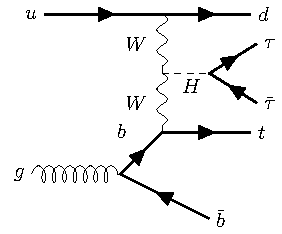
\includegraphics[width=0.45\textwidth]{/cephfs/user/s6chkirf/feynman_diagrams/tHq_tautau}\\
      \includegraphics[width=0.45\textwidth]{/cephfs/user/s6chkirf/feynman_diagrams/tHq_WW}
      \includegraphics[width=0.45\textwidth]{/cephfs/user/s6chkirf/feynman_diagrams/tHq_ZZ}
      \begin{itemize}
        \item n-jets: 2 (b-jets: \textbf{1})
        \item b-jet WP: 70 DL1r
        \item nLeptons \& nTaus: \bf{$1e / \mu~2\tau_{\text{had}}$}
        \item $E_{\text{T,miss}}$: no cut (to \SI{800}{GeV})
      \end{itemize}
    \end{column}
    \begin{column}{0.7\textwidth}
      \vspace*{-0.05\textwidth}
      \begin{itemize}
        \footnotesize
        \item jets:
        \vspace*{-0.02\textwidth}
        \begin{itemize}
          \footnotesize
          \item $p_T>\SI{35}{GeV}$
          \item $|\eta|<4.5$
          \item EMPFlow
        \end{itemize}
        \item electrons:
        \vspace*{-0.02\textwidth}
        \begin{itemize}
          \footnotesize
          \item $p_T>\SI{20}{GeV}$ leading \SI{27}{GeV}
          \item $|\eta|<2.5$ not in 1.37 - 1.52
          \item WP: LooseAndBLayerLH ; \\isolation: no requirement
        \end{itemize}
        \item muons:
        \vspace*{-0.02\textwidth}
        \begin{itemize}
          \footnotesize
          \item $p_T>\SI{20}{GeV}$ leading \SI{27}{GeV}
          \item $0.01<|\eta|<2.5$
          \item WP: Loose ; isolation: no requirement
        \end{itemize}
        \item taus:
        \vspace*{-0.02\textwidth}
        \begin{itemize}
          \footnotesize
          \item $p_T>\SI{20}{GeV}$ leading \SI{27}{GeV}
          \item $|\eta|<2.5$ not in 1.37 - 1.52
          \item WP: RNNLoose
          \item ASG recommended OLR ($\tau_{had}$ remove jets)
        \end{itemize}
      \end{itemize}
    \end{column}
  \end{columns}
\end{frame}
  

\section*{Comparison 1}
\begin{frame}{G4 to G4 with frozen shower}
    \begin{columns}
        \begin{column}{0.5\textwidth}
            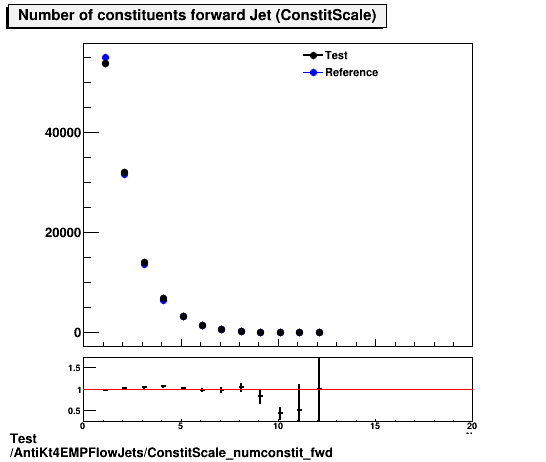
\includegraphics[width=0.85\textwidth]{1r_numconstit_constit}
        \end{column}
        \begin{column}{0.5\textwidth}
            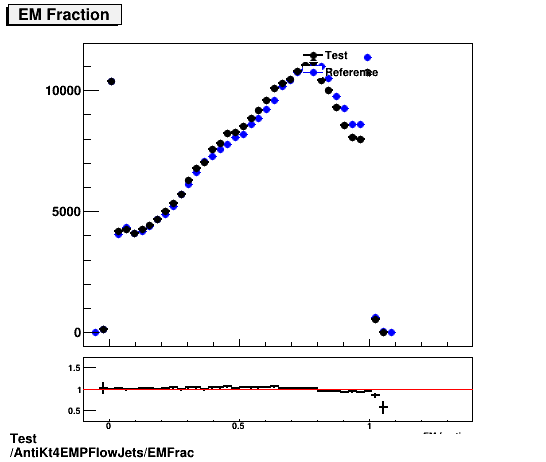
\includegraphics[width=0.85\textwidth]{1r_EMFrac}
        \end{column}
    \end{columns}
        \begin{itemize}
            \item Good agreement between G4 and G4 without frozen shower
            \item Number of constituents and kinematics look good
            \item Shape differences for the EMFrac
        \end{itemize}
\end{frame}

\section*{Comparison 2}
\begin{frame}{AF to G4 with frozen shower}
    \begin{columns}
        \begin{column}{0.5\textwidth}
            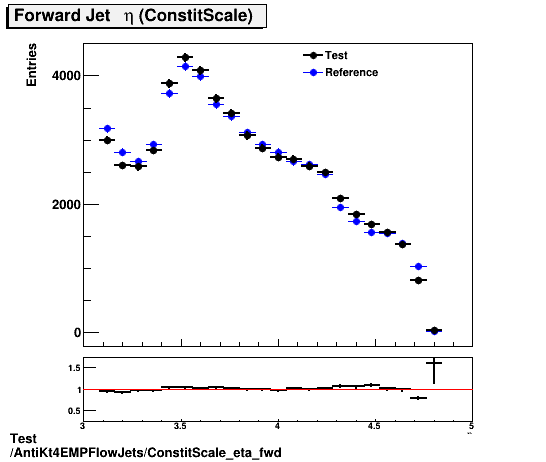
\includegraphics[width=0.85\textwidth]{2r_eta_constit}
        \end{column}
        \begin{column}{0.5\textwidth}
            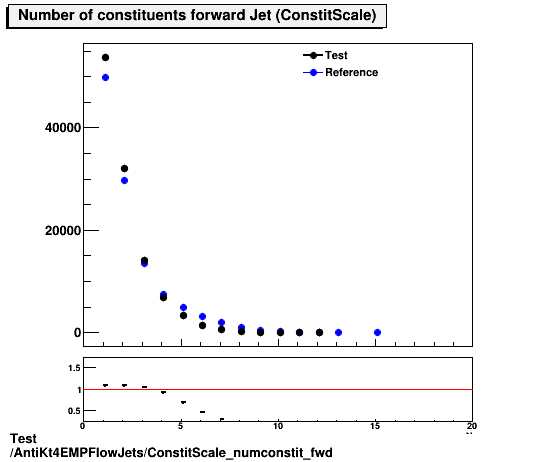
\includegraphics[width=0.85\textwidth]{2r_numconstit_constit}
        \end{column}
    \end{columns}
    \begin{itemize}
        \item A few plots are marked red. Nothing shows large disagreements.
        \item Kinematics have acceptable agreement.
    \end{itemize}
\end{frame}
\section*{Comparison 3}
\begin{frame}{AF to G4 without frozen shower, red plots}
    \begin{columns}
        \begin{column}{0.5\textwidth}
            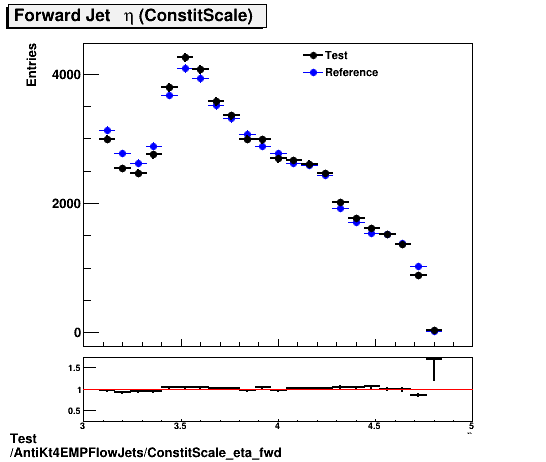
\includegraphics[width=0.75\textwidth]{3r_eta_constit}
            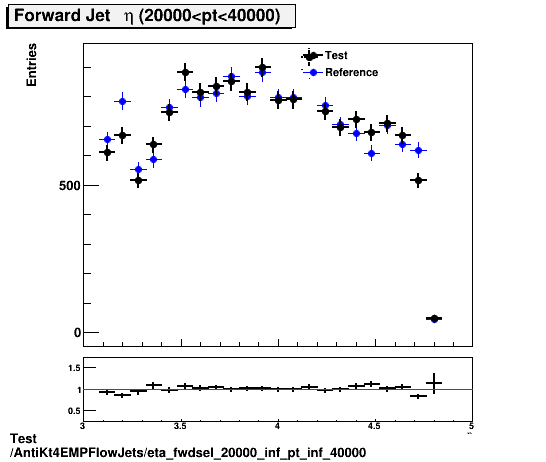
\includegraphics[width=0.75\textwidth]{3r_eta_highpt}
        \end{column}
        \begin{column}{0.5\textwidth}
            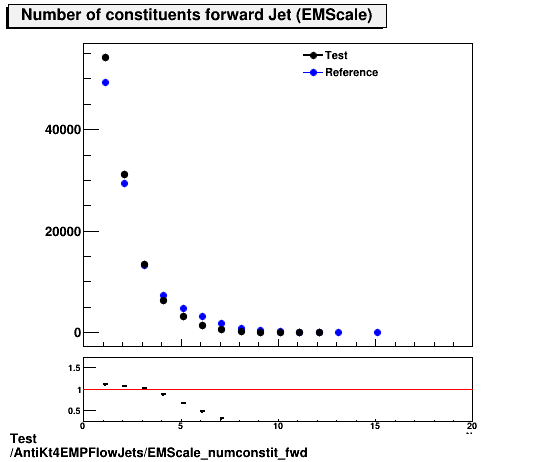
\includegraphics[width=0.75\textwidth]{3r_numconstit_EM}
            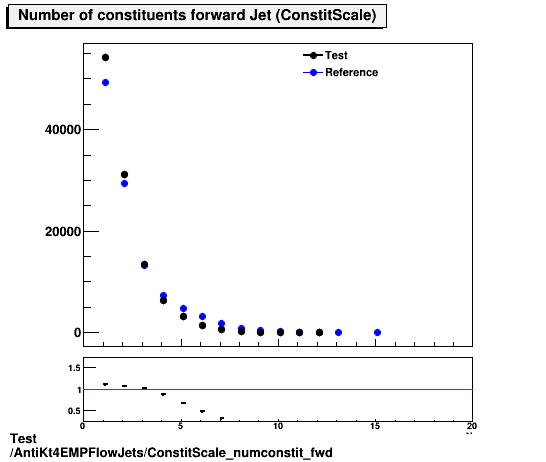
\includegraphics[width=0.75\textwidth]{3r_cumconstit_constit}
        \end{column}
    \end{columns}
\end{frame}

\begin{frame}{AF to G4 without frozen shower, decent agreement}
    \begin{columns}
        \begin{column}{0.5\textwidth}
            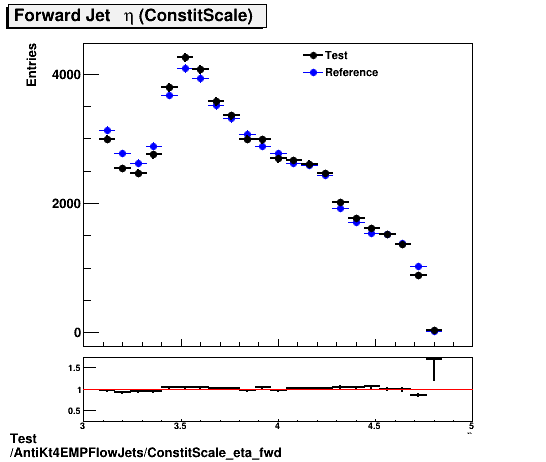
\includegraphics[width=0.85\textwidth]{3r_eta_constit}
        \end{column}
        \begin{column}{0.5\textwidth}
            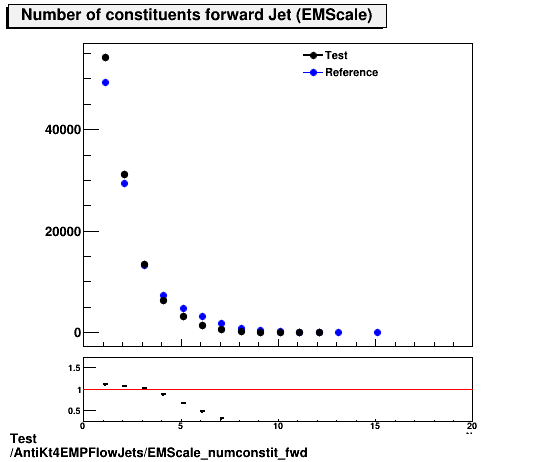
\includegraphics[width=0.85\textwidth]{3r_numconstit_EM}
        \end{column}
    \end{columns}
    \begin{itemize}
        \item The number of constituents in the forward region is slightly off but the kinematics look ok
    \end{itemize}
\end{frame}

%\begin{frame}{Sources}

%\printbibliography
    
%\end{frame}






\end{document}